\documentclass{beamer}
\mode<presentation>
\usepackage{tikz}
\usepackage{multimedia}
\setbeamertemplate{caption}{\insertcaption}
\renewcommand{\thefootnote}{\fnsymbol{footnote}}
% \usepackage{pdfpc-movie}
\usepackage{graphicx} %The mode "LaTeX => PDF" allows the following formats: .jpg  .png  .pdf  .mps
% \usepackage{media9}
\usetikzlibrary{arrows, shapes.geometric,matrix,positioning,graphs,quotes}
\title{Class 8 Draft Textbook Chapter: Sound}
\author[dishajk]{Disha Kuzhively}
\institute{International Centre for Theoretical Sciences - TIFR, Bangalore}
\date[Chennai]{\today\\{\texttt disha.jk@icts.res.in} }
\begin{document}
% \begin{frame}
%     \titlepage
% \end{frame}
\begin{frame}
    \frametitle{Outline}
    \tableofcontents
\end{frame}
\section{Transdisciplinary approach}
\begin{frame}
  \frametitle{Transdisciplinary approach}
\only<1-2>{
  Connecting concepts across disciplines to create a more coherent and meaningful learning experience.
}
\only<2>{
   \begin{block}{Example: Understanding the Human Ear}
    The human ear is usually introduced as a topic in \alert{Biology}.

    In a \alert{Physics} chapter on Sound, the ear can be introduced to help students understand how sound is detected and heard.

    This connects the physics of sound with the biology of hearing, showing students that scientific ideas do not exist in isolated subjects.
  \end{block}
}
\only<3>{
  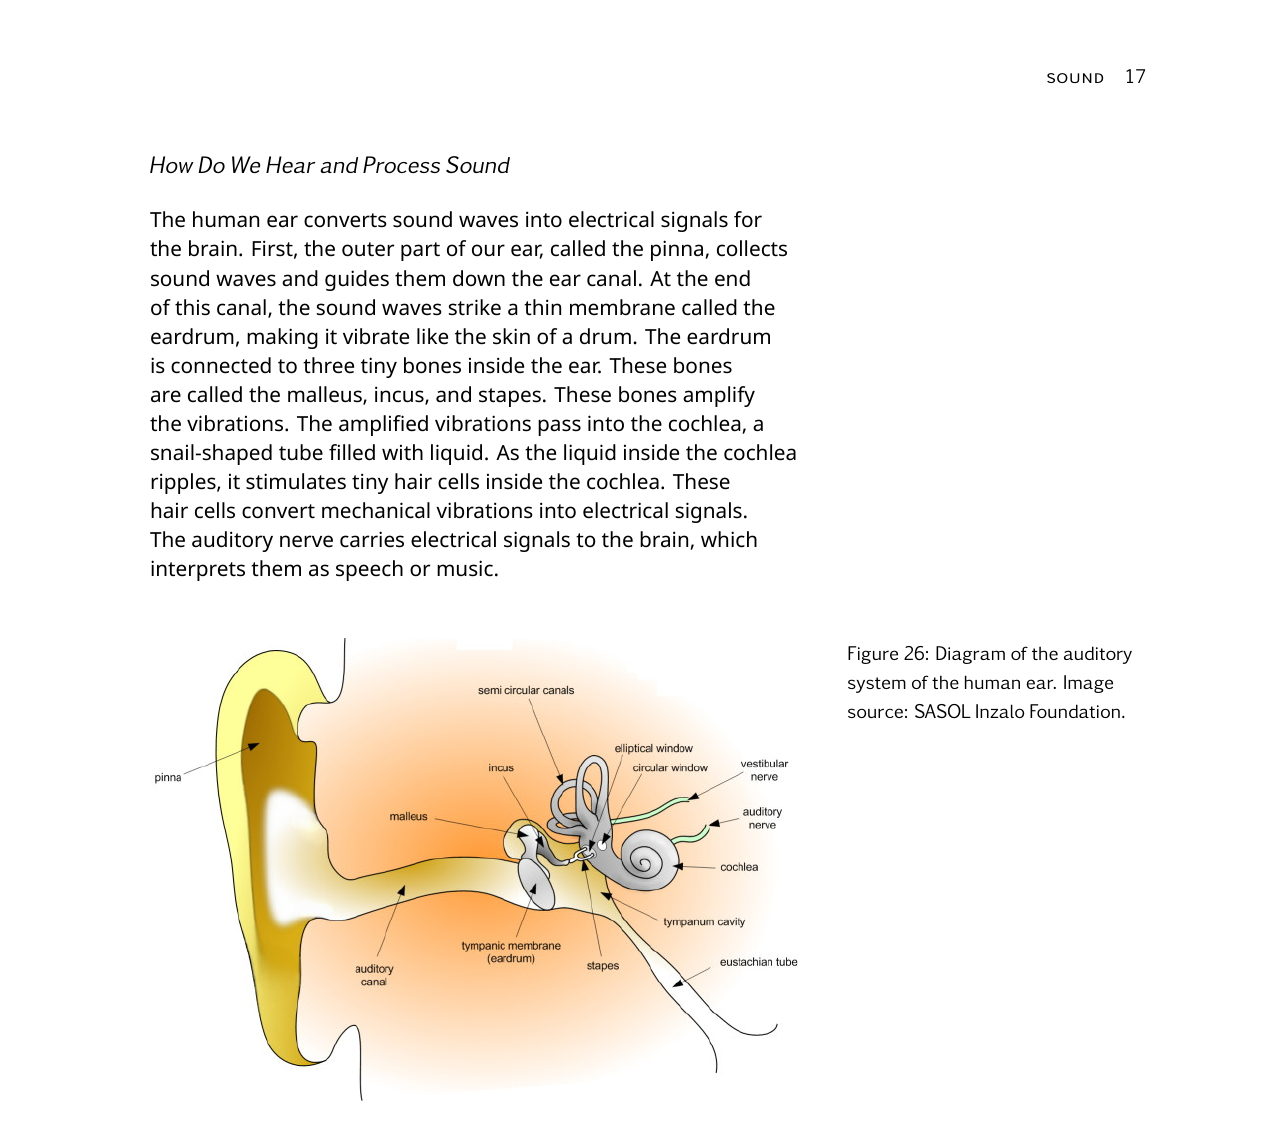
\includegraphics[height=0.8\textheight]{transdisc}
}
\end{frame}
\section{Computational Thinking, Analysis \& Problem Solving}
\begin{frame}
  \frametitle{Computational Thinking, Analysis \& Problem Solving}
  \only<1-2>{
    The textbook embeds questions and problem-solving directly into the learning material, encouraging students to observe, analyse, identify patterns, and reason with data as they build the concept.
  }
  \only<2>{
  \begin{block}{Example: Understanding Frequency}
    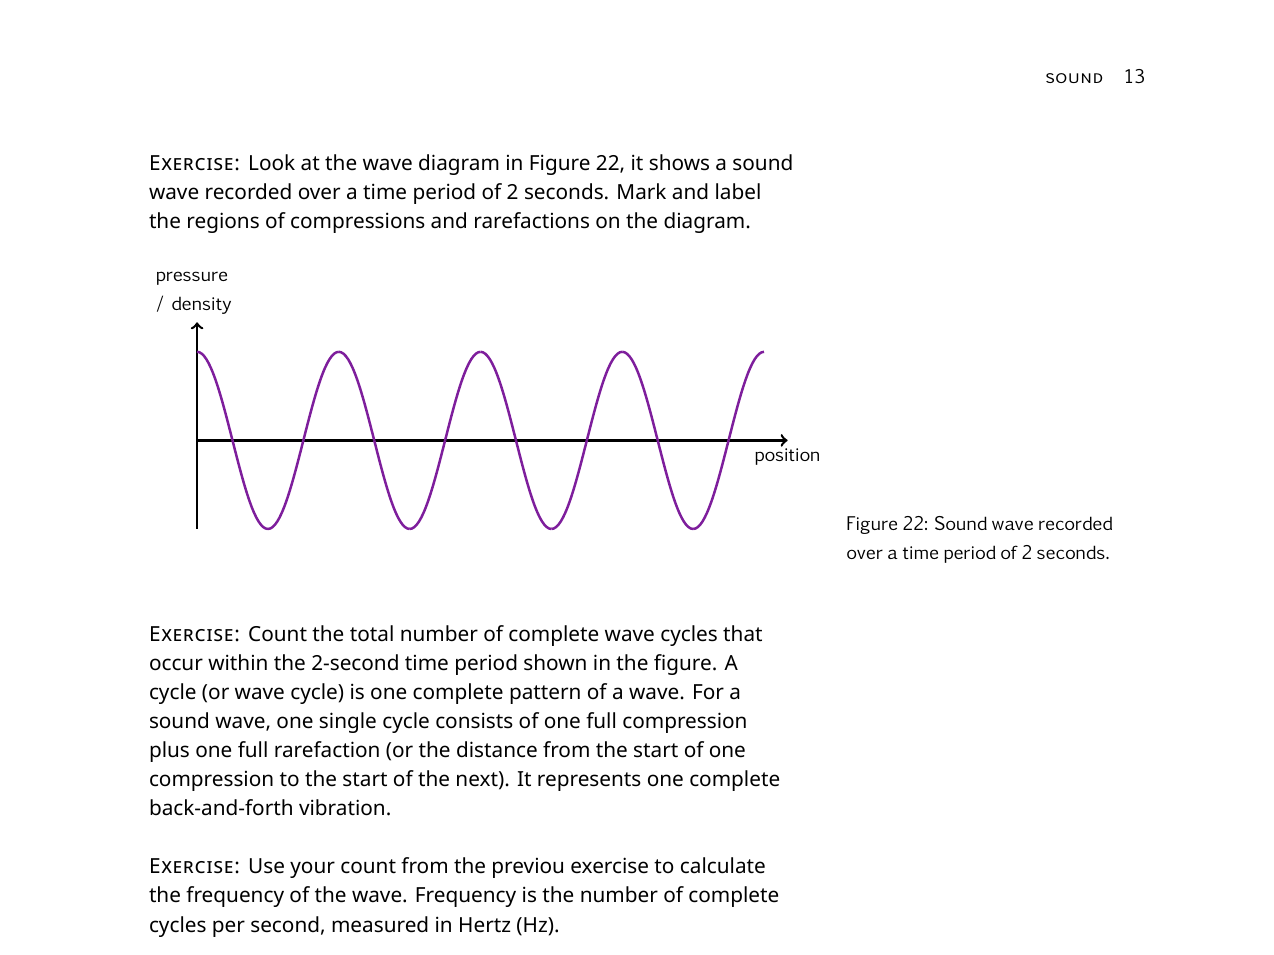
\includegraphics[height=0.7\textheight]{compthink}
  \end{block}
  }
\end{frame}
\section{Technology-Enabled Education}
\begin{frame}
  \frametitle{Technology-Enabled Education}
  \only<1-3>{
    Using digital tools to extend what students can observe, measure, and investigate.
  }
  \only<2>{
\begin{block}{Example: Investigating Pitch}
Students first explore pitch through the Singing Pipe and Glass activity.

With the help of a smartphone and the \alert{Phyphox} app, the teacher can measure the frequency of the sounds produced.

Students can then compare their observations with the measured frequencies.
\end{block}
}
\only<3>{
    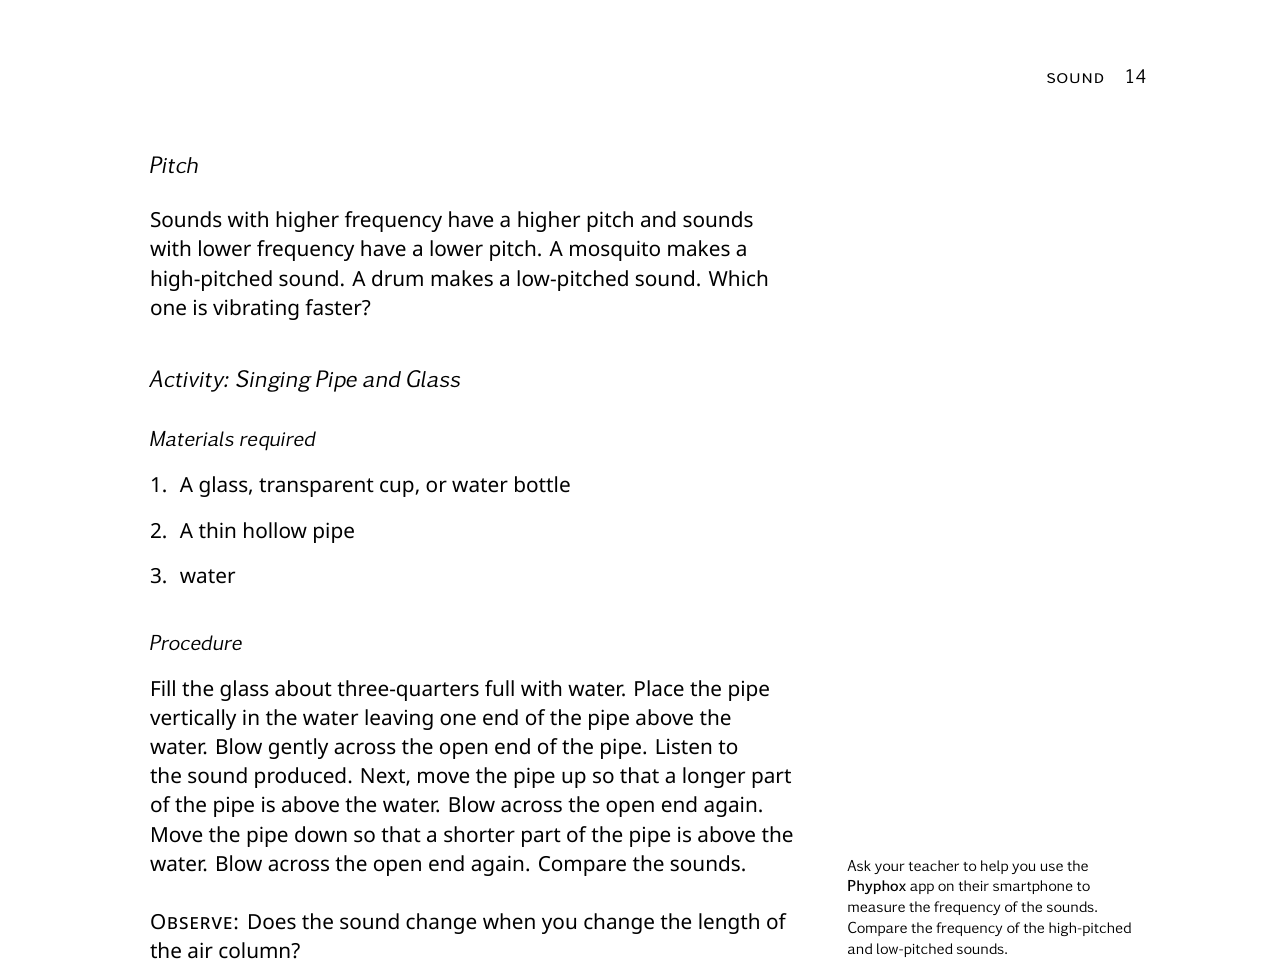
\includegraphics[height=0.7\textheight]{techuse}
}
\end{frame}
\section{Connecting Concepts to Everyday Life}
\begin{frame}
  \frametitle{Connecting Concepts to Everyday Life}
  \only<1-3>{
    Learning becomes more meaningful when students can connect scientific ideas to things they experience, observe, and use in everyday life.
  }
  \only<2>{
    \begin{block}{Example: How Do We Form Different Sounds?}
      In the chapter on Sound, students can explore how the sounds they use in everyday speech are produced.
    \end{block}
  }
  \only<3>{
    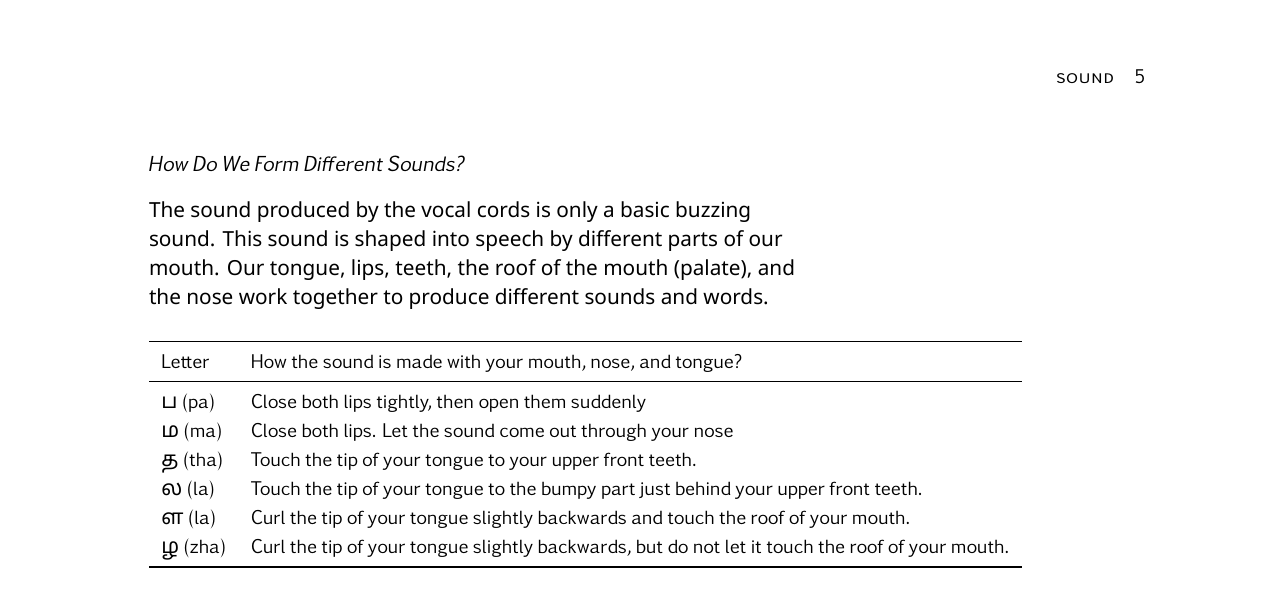
\includegraphics[width=0.9\textwidth]{everydaylife}
  }
\end{frame}
\section{Developing Sensitivity and Scientific Temper}
\begin{frame}
\frametitle{Developing Sensitivity and Scientific Temper}  
\only<1-3>{
  Science education should help students understand not only how the world works, but also how their knowledge can shape the way they live and act in it.
}
\only<2>{
  \begin{block}{Example: Noise Pollution \& Hearing Loss}
    After learning about sound, students are also taught about noise pollution, and how it affects people and other living beings.
  \end{block}
}
\only<3>{
  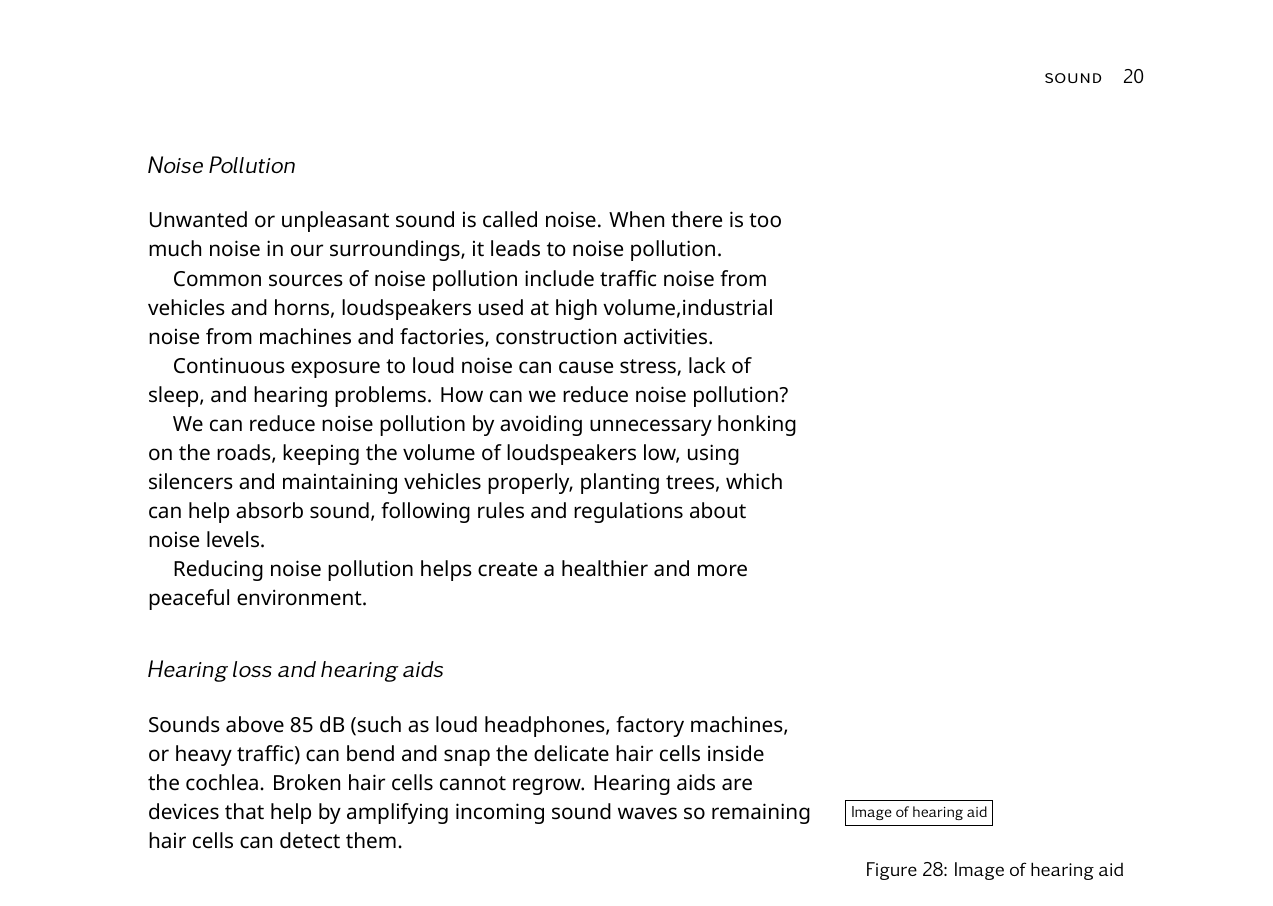
\includegraphics[height=0.7\textheight]{sensitivity}
}
\end{frame}
\end{document}
